\documentclass[a4paper,12pt]{article}
\usepackage[a4paper,top=1.3cm,bottom=2cm,left=1.5cm,right=1.5cm,marginparwidth=0.75cm]{geometry}
\usepackage{cmap}
\usepackage{mathtext}
\usepackage[T2A]{fontenc}
\usepackage[utf8]{inputenc}
\usepackage[english,russian]{babel}
\usepackage{siunitx}

\usepackage{graphicx}

\usepackage{wrapfig}
\usepackage{tabularx}
\usepackage{multirow}

\usepackage{hyperref}
\usepackage[rgb]{xcolor}
\hypersetup{
colorlinks=true,urlcolor=blue
}
\usepackage{amsmath,amsfonts,amssymb,amsthm,mathtools}
\usepackage{icomma}
\mathtoolsset{showonlyrefs=false}
\usepackage{euscript}
\usepackage{mathrsfs}
\DeclareMathOperator{\sgn}{\mathop{sgn}}
\newcommand*{\hm}[1]{#1\nobreak\discretionary{}
{\hbox{$\mathsurround=0pt #1$}}{}}

%%% Заголовок
\author{Макаров Лев Евгеньевич}
\title{Лабораторная работа №1.3.3

Измерение вязкости воздуха по течению в тонких трубках
}
\date{\today}

\begin{document}

\begin{titlepage}
	\begin{center}
		{\large МОСКОВСКИЙ ФИЗИКО-ТЕХНИЧЕСКИЙ ИНСТИТУТ (НАЦИОНАЛЬНЫЙ ИССЛЕДОВАТЕЛЬСКИЙ УНИВЕРСИТЕТ)}
	\end{center}
	\begin{center}
		{\large Физтех-школа фотоники, электроники и молекулярной физики}
	\end{center}
	
	
	\vspace{4.5cm}
	{\huge
		\begin{center}
			{\bf Отчёт о выполнении лабораторной работы 1.3.3}\\
			Измерение вязкости воздуха по течению в тонких трубках
		\end{center}
	}
	\vspace{2cm}
	\begin{flushright}
		{\LARGE Автор:\\ Макаров Лев Евгеньевич \\
			\vspace{0.2cm}
			Б04-306}
	\end{flushright}
	\vspace{8cm}
	\begin{center}
		Долгопрудный 2024
	\end{center}
\end{titlepage}

\section{Введение}

\textbf{Цель работы:} 
\begin{enumerate}
	\item экспериментально исследовать свойства течения газов по тонким трубкам при различных числах Рейнольдса
    \item выявить область применения закона Пуазейля и с его помощью определить коэффициент вязкости воздуха
\end{enumerate}

\textbf{В работе используются:} 
\begin{itemize}
    \item система подачи воздуха (компрессор, поводящие трубки)
    \item газовый счетчик барабанного типа
    \item спиртовой микроманометр с регулируемым наклоном
    \item набор трубок различного диаметра с выходами для подсоединения микроманометра
    \item секундомер
\end{itemize}
\medskip

\section{Теоретические сведения}

Рассмотрим движение вязкой жидкости или газа по трубке круглого сечения. При малых скоростях потока движение оказывается ламинарным (слоистым), скорости частиц меняются по радиусу и направлены вдоль оси трубки. С увеличением скорости потока движение становится турбулентным, а слои перемешиваются. При турбулентном движении скорость в каждой точке быстро меняет величину и направление, сохраняется только средняя величина скорости.

Характер движения газа (или жидкости) в трубке определяется безразмерным числом Рейнольдса:

\begin{equation}\label{1}
    Re = \frac{vr\rho}{\eta}
\end{equation}


где $v$ -- скорость потока, $r$ -- радиус трубки, $\rho$ -- плотность движущейся среды, $\eta$ -- её вязкость. В гладких трубах круглого сечения переход от ламининарного движения к турбулентному происходит при $Re \approx 1000$.

При ламинарном течении объем газа $V$, протекающий за время $t$ по трубе длиной $l$, определяется формулой Пуазейля:

\begin{equation}\label{2}
	Q = \frac{\pi r^4}{8 \Delta l \eta}(P_1 - P_2)
\end{equation}

В этой формуле $P_1 - P_2$ -- разность давлений в двух выбранных сечениях 1 и 2, расстояние между которыми равно $\Delta l$. Величину $Q$ обычно называют расходом. Формула (1) позволяет определять вязкость газа по его расходу.

Отметим условия, при которых справедлива формула (1). Прежде всего необходимо, чтобы с достаточным запасом выполнялось неравенство $Re < 1000$. Необходимо также, чтобы при течении не происходило существенного изменения удельного объёма газа (при выводе формулы удельный объём считался постоянным). Для жидкости это предположение выполняется практически всегда, а для газа --- лишь в тех случаях, когда перепад давлений вдоль трубки мал по сравнению с самим давлением. В нашем случае давление газа равно атмосферному ($10^3$ см вод. ст.), а перепад давлений составляет не более 10 см вод. ст., т. е. менее 1\% от атмосферного. Формула (1) выводится для участков трубки, на которых закон распределения скоростей газа по сечению не меняется при двидении вдоль потока.

% \begin{wrapfigure}{l}{0.4\textwidth}
%     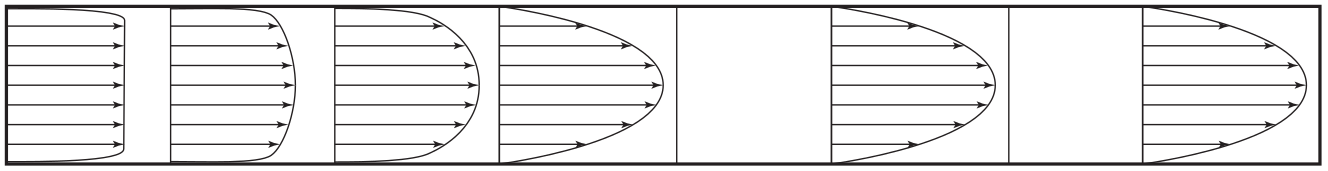
\includegraphics[width=1\linewidth]{potok.png}
%     \centering
%     \caption{Формирование потока газа в трубке круглого сечения}
%     \label{potok}
% \end{wrapfigure}
\begin{figure}
    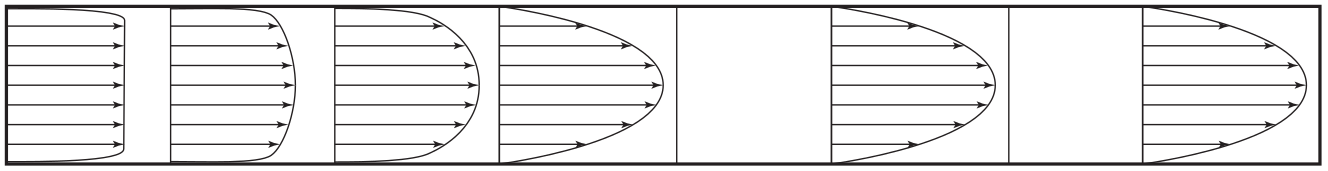
\includegraphics[width=1\linewidth]{potok.png}
    \centering
    \caption{Формирование потока газа в трубке круглого сечения}
    \label{potok}
\end{figure}

При втекании газа в трубку из большого резервуара скорости слоёв вначале постоянны по всему направлению. По мере продвижения газа по трубке картина распределения скоростей меняется, так как сила трения о стенку тормозит прилежащие к ней оси. Характерное для ламинарного течения параболическое распределение скоростей устанавливается на некотором расстоянии $a$ от входа в трубку, которое зависит от радиуса трубки $r$ и числа Рейнольдса по формуле 

\begin{equation}
    l_\text{уст} \approx 0.2rRe
\end{equation}

Градиент давления на участке формирования потока оказывается больше, чем на участке с установившимся ламинарным течением, что позволяет разделить эти участки экспериментально. Формула (2) даёт возможность оценить дину участка формирования.

\section{Оборудование и экспериментальные погрешности}

\textbf{Секундомер:} $\sigma_\text{s} = 0,6$ с \\
\textbf{Спиртовый микрометр:} $\sigma_\text{м} = $  \\
\textbf{Газовый счётчик:} $\sigma_\text{г} = $ 

\subsection*{Эксперементальная установка}

Схема экспериментальной установки изображена на рис. \ref{ustan}. Поток воздуха под давлением, немного превышающим атмосферное, поступает через газовый счётчик в тонкие металлические трубки. Воздух нагнетается компрессо-
ром, интенсивность его подачи регулируется краном К. Трубки снабжены съёмными заглушками на концах и рядом миллиметровых отверстий, к которым можно подключать микроманометр. В рабочем состоянии открыта заглушка на одной (рабочей) трубке, микроманометр подключён к двум её выводам, а все остальные отверстия плотно закрыты пробками.

Перед входом в газовый счётчик установлен водяной U-образный манометр. Он служит для измерения давления газа на входе, а также предохраняет счётчик от выхода из строя. При превышении максимального избыточного давления на входе счётчика ($\sim$ 30 см вод. ст.) вода выплёскивается из трубки в защитный баллон Б, создавая шум и привлекая к себе внимание экспериментатора.

\begin{figure}[!h]
    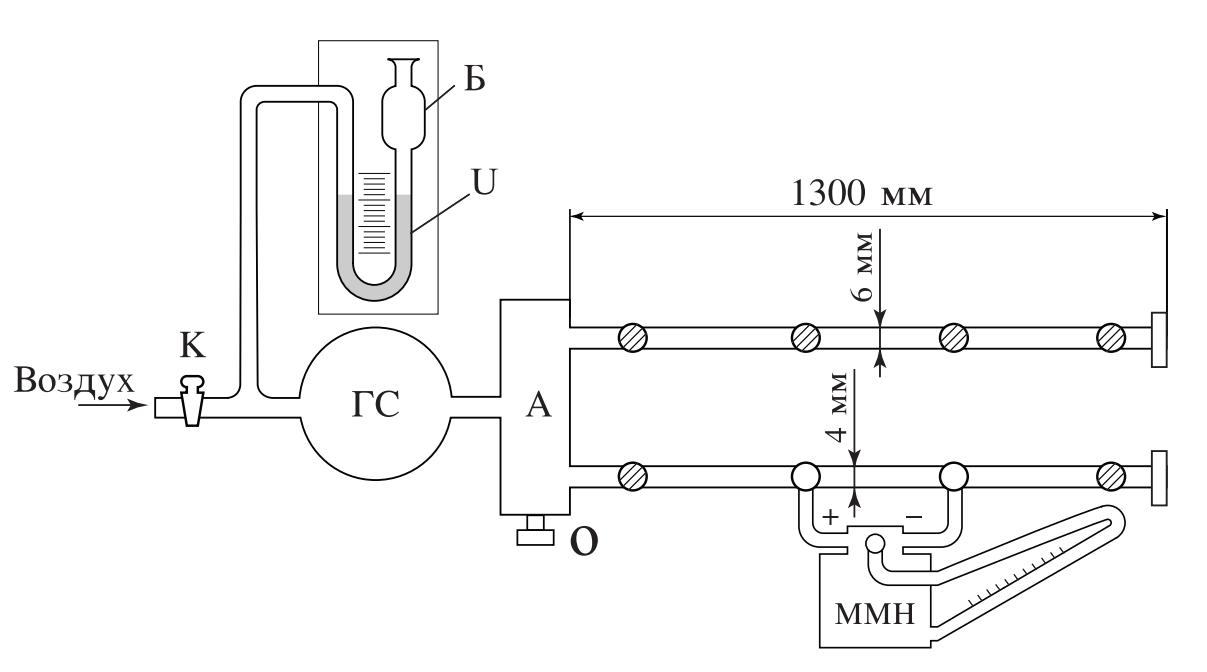
\includegraphics[width=0.8\linewidth]{ustan.png}
    \centering
    \caption{Формирование потока газа в трубке круглого сечения}
    \label{ustan}
\end{figure}

\newpage

\section{Результаты измерений и обработка данных}

\subsection{Подготовка установки}

Ознакомимся с устройством, проверим, что предварительная настройка оборудования была проведена правильно.

Ознакомимся с измерительными шкалами приборов.

\subsection{Запуск установки}

Запустим установку и убедимся, что всё оборудование работает корректно.

Подсоединим манометр к двум соседним выводам трубки с диаметром $d_1 = (3,90 \pm 0,05)$ мм. Убедимся, что все отверстия плотно завинчены пробками (кроме выходного). Убедимся, что кран К закрыт, и включим компрессор. Дальше создадим небольшой поток воздуха и убедимся, что показания микроманометра стабильны.

\subsection{Измерение параметров}

Запишем параметры трубок:

\begin{equation*}
    d_1 = (3,90 \pm 0,05) \ \text{мм}, \ \ \ d_2 = (5,25 \pm 0,05) \ \text{мм}
\end{equation*}

Теперь измерим параметры окружающей среды:

\begin{equation*}
    T_0 = (297,7 \pm 0,3) \ \text{К}, \ \ \ \varphi = 16,8 \%, \ \ \ P_0 = 100420 \ \text{Па}
\end{equation*}

Вычислим плотность воздуха по этим данным $\rho = \mu P_0 / R T_0 \approx 1,18 \ \text{кг}/\text{м}^3$.

% Погрешность измерения плотности можно вычислить по формуле:

% \begin{equation}
%     \sigma_\rho = 
% \end{equation}

\subsection{Предварительные расчёты}
\label{p:4}

Оценим критеческое значение расхода $Q_\text{кр}$:

\begin{equation*}
    Re_\text{кр} = \frac{\overline{u} r \rho}{\eta} = \frac{Q_\text{кр}}{\pi r} \frac{\rho}{\eta} \implies 
\end{equation*}
\begin{equation*}
    \implies Q_\text{кр} = \frac{\pi r \eta Re_\text{кр}}{\rho} = \frac{R T_0 \pi d_1 \eta Re_\text{кр}}{2 \mu P_0} = \frac{8,31 \cdot 297,7 \cdot 3,14 \cdot 3,90 \cdot 10^{-3} \cdot 2 \cdot 10^{-5} \cdot 1000}{2 \cdot 29 \cdot 10^{-3} \cdot 100420} 60 \approx 6 \ \frac{\text{л}}{\text{мин}} 
\end{equation*}

Рассчитаем критический перепад давления в трубе $\Delta P_\text{кр}$ по формуле Пуазейля:

\begin{equation*}
    \Delta P_\text{кр} = \frac{Q_\text{кр} 8 \eta l }{\pi r^4} = \frac{0,0001 \cdot 8 \cdot 2 \cdot 10^{-5} \cdot 0,5}{3,14 \cdot (3,90 \cdot 10^{-3} / 2)^4} \approx 176 \ \text{Па}
\end{equation*}

Оценим длину $l_\text{уст}$

\begin{equation*}
    l_\text{уст} = 0,2 r \cdot Re = 0,2 \cdot \frac{3,90}{2} \cdot 1000 \approx 390 \ \text{мм}
\end{equation*}

\subsection{Нахождение границы перехода от ламинарного течения к турбулентному}

Меняя расход с помощью крана К визуально найдём границу перехода о ламинарного течения к турбулентному.


\subsection{Подборка параметров измерения расхода}

Подберём параметры измерения расхода так, чтобы относительная погрешность составила не более, чем 1 \%. Для этого нужно проводить измерения не менее 30 секунд при любом расходе.

\subsection{Измерение зависимости перепада давления от расхода}

Измерим зависимость перепада давления от расхода. Для этого будем постепенно увеличивать значение расхода до тех пор, пока течение остаётся ламинарным. Когда течение станет турбулентным замерим ещё несколько точек. Все результаты измерения занесём в таблицу \ref{table:q-1}.

\begin{table}[!h]
    \centering
    \begin{tabular}{|l|l|l|l|}
    \hline
        $N$ & $h$, мм & $Q$, л/мин & $\Delta P$, Па  \\ \hline
        1 & 5 & 0,341 & 7,9  \\ \hline
        2 & 10 & 0,683 & 15,9  \\ \hline
        3 & 15 & 1,000 & 23,8  \\ \hline
        4 & 20 & 1,353 & 31,8  \\ \hline
        5 & 25 & 1,667 & 39,7  \\ \hline
        6 & 30 & 1,989 & 47,6  \\ \hline
        7 & 35 & 2,286 & 55,6  \\ \hline
        8 & 40 & 2,636 & 63,5  \\ \hline
        9 & 45 & 2,937 & 71,5  \\ \hline
        10 & 50 & 3,245 & 79,4  \\ \hline
        11 & 55 & 3,553 & 87,4  \\ \hline
        12 & 60 & 3,864 & 95,3  \\ \hline
        13 & 65 & 4,131 & 103,2  \\ \hline
        14 & 70 & 4,431 & 111,2  \\ \hline
        15 & 75 & 4,712 & 119,1  \\ \hline
        16 & 80 & 4,981 & 127,1  \\ \hline
        17 & 90 & 5,317 & 142,9  \\ \hline
        18 & 100 & 5,506 & 158,8  \\ \hline
        19 & 110 & 5,685 & 174,7  \\ \hline
        20 & 120 & 5,897 & 190,6  \\ \hline
        21 & 130 & 6,108 & 206,5  \\ \hline
        22 & 140 & 6,308 & 222,4  \\ \hline
        23 & 150 & 6,501 & 238,2  \\ \hline
        24 & 160 & 6,656 & 254,1  \\ \hline
        25 & 170 & 6,865 & 270,0  \\ \hline
        26 & 180 & 7,019 & 285,9  \\ \hline
        27 & 190 & 7,195 & 301,8  \\ \hline
        28 & 200 & 7,394 & 317,6  \\ \hline
        29 & 210 & 7,542 & 333,5  \\ \hline
    \end{tabular}\caption{\textit{Измерение зависимости давления от расхода для первой трубы}}\label{table:q-1}
\end{table}

% \begin{table}[!ht]
%     \centering
%     \begin{tabular}{|l|l|l|l|l|l|l|l|l|l|l|l|l|l|l|l|l|l|l|l|l|l|l|l|l|l|l|l|l|l|}
%     \hline
%         $№$ & 1 & 2 & 3 & 4 & 5 & 6 & 7 & 8 & 9 & 10 & 11 & 12 & 13 & 14 & 15 & 16 & 17 & 18 & 19 & 20 & 21 & 22 & 23 & 24 & 25 & 26 & 27 & 28 & 29 \\ \hline
%         $h,\;мм$ & 5 & 10 & 15 & 20 & 25 & 30 & 35 & 40 & 45 & 50 & 55 & 60 & 65 & 70 & 75 & 80 & 90 & 100 & 110 & 120 & 130 & 140 & 150 & 160 & 170 & 180 & 190 & 200 & 210 \\ \hline
%         $Q,\;л/мин$ & 0,341 & 0,683 & 1,000 & 1,353 & 1,667 & 1,989 & 2,286 & 2,636 & 2,937 & 3,245 & 3,553 & 3,864 & 4,131 & 4,431 & 4,712 & 4,981 & 5,317 & 5,506 & 5,685 & 5,897 & 6,108 & 6,308 & 6,501 & 6,656 & 6,865 & 7,019 & 7,195 & 7,394 & 7,542 \\ \hline
%         $\Delta P,\;Па$ & 7,9 & 15,9 & 23,8 & 31,8 & 39,7 & 47,6 & 55,6 & 63,5 & 71,5 & 79,4 & 87,4 & 95,3 & 103,2 & 111,2 & 119,1 & 127,1 & 142,9 & 158,8 & 174,7 & 190,6 & 206,5 & 222,4 & 238,2 & 254,1 & 270,0 & 285,9 & 301,8 & 317,6 & 333,5 \\ \hline
%     \end{tabular}\caption{\textit{Измерение зависимости давления от расхода для первой трубы}}\label{table:q-1}
% \end{table}

\subsection{Измерение распределения давления вдоль трубы}
\label{p:8}

Измерим распределение давления газа вдоль трубки $P(x)$. Установим поток воздуха так, чтобы он сохранл ламинарность. Не меняя расхода, последовательно будем подсоединять микроманометр к каждой соседней паре выходов и измерить разницу давления. Результаты измерений запишем в таблицу \ref{table:p-1}.

\begin{table}[!h]
    \centering
    \begin{tabular}{|l|r|r|r|r|}
    \hline
        $N$ & $x$, см & $L$, см & $h$, мм & $\Delta P$, Па \\ \hline
        1 & 81 & 50 & 50 & 79,4 \\ \hline
        2 & 41 & 40 & 40 & 63,5 \\ \hline
        3 & 11 & 30 & 30 & 47,6 \\ \hline
        4 & 0 & 11 & 38 & 60,4 \\ \hline
    \end{tabular}\caption{\textit{Измерение распределения давления вдоль первой трубы}}\label{table:p-1}
\end{table}

\subsection{Измерения для второй трубы}

Проведём измерения, аналогичные пунктам \ref{p:4}-\ref{p:8}, для второй трубы с диаметром $d_2 = (5,25 \pm 0,05)$ мм. Все результаты измерений запишем в таблицы \ref{table:q-2} и \ref{table:p-2} соответственно.

\begin{table}[!ht]
    \centering
    \begin{tabular}{|l|l|l|l|}
    \hline
        $N$ & $h$, мм & $Q$, л/мин & $\Delta P$, Па  \\ \hline
        1 & 9 & 1,969 & 14,3 \\ \hline
        2 & 14 & 3,106 & 22,2 \\ \hline
        3 & 19 & 4,171 & 30,2 \\ \hline
        4 & 24 & 5,223 & 38,1 \\ \hline
        5 & 29 & 6,293 & 46,1 \\ \hline
        6 & 34 & 7,226 & 54,0 \\ \hline
        7 & 44 & 7,838 & 69,9 \\ \hline
        8 & 54 & 8,311 & 85,8 \\ \hline
        9 & 64 & 8,748 & 101,6 \\ \hline
        10 & 74 & 9,326 & 117,5 \\ \hline
        11 & 84 & 9,931 & 133,4 \\ \hline
        12 & 94 & 10,497 & 149,3 \\ \hline
        13 & 104 & 11,101 & 165,2 \\ \hline
        14 & 114 & 11,715 & 181,1 \\ \hline
        15 & 124 & 12,303 & 196,9 \\ \hline
        16 & 134 & 12,760 & 212,8 \\ \hline
        17 & 144 & 13,287 & 228,7 \\ \hline
        18 & 154 & 13,795 & 244,6 \\ \hline
        19 & 164 & 14,298 & 260,5 \\ \hline
        20 & 174 & 14,785 & 276,4 \\ \hline
        21 & 184 & 15,260 & 292,2 \\ \hline
        22 & 194 & 15,733 & 308,1 \\ \hline
        23 & 204 & 16,084 & 324,0 \\ \hline
        24 & 214 & 16,434 & 339,9 \\ \hline
    \end{tabular}\caption{\textit{Измерение зависимости давления от расхода для второй трубы}}\label{table:q-2}
\end{table}

\begin{table}[!ht]
    \centering
    \begin{tabular}{|l|l|l|l|l|}
    \hline
        1 & 80,5 & 50 & 20 & 31,8 \\ \hline
        2 & 40,5 & 40 & 17 & 27,0 \\ \hline
        3 & 10,5 & 30 & 13 & 20,6 \\ \hline
        4 & 0 & 10,5 & 17 & 27,0 \\ \hline
    \end{tabular}\caption{\textit{Измерение распределения давления вдоль второй трубы}}\label{table:p-2}
\end{table}

\clearpage

\subsection{Измерение зависимости расхода от радиуса при выбранном градиенте}\label{p:10}

Данный пункт работы не выполнялся.

\subsection{График зависимости расхода от перепада давления}

Построим график зависимости расхода от перепада давления $Q(\Delta P)$. Зависимость на ламинарном и турбулентном участках должна быть прямой (по отдельности), поэтому для каждого участка можем воспользоваться МНК для нахождения наилучшей прямой. В данном случае $x = \Delta P$, а $y = Q$. Для аппроксимации наилучшей прямой воспользуемся формулой:

\begin{equation}\label{eq:mnk}
    k = \frac{\langle xy\rangle - \langle x \rangle \langle y \rangle}{\langle x^2 \rangle - \langle x \rangle^2},
    \ \text{а} \ \  b = \langle y \rangle - k\langle x \rangle
\end{equation}

Погрешности для $k$ и $b$ рассчитываются по формулам:

\begin{equation}
    \sigma_k = \frac{1}{\sqrt{n}} \sqrt{\frac{\langle y^2 \rangle - \langle y \rangle^2}{\langle x^2 \rangle - \langle x \rangle^2} - k^2}
\end{equation}

\begin{equation}
    \sigma_b = \sigma_k\sqrt{\langle x^2 \rangle - \langle x \rangle^2}
\end{equation}

Посчитаем значения МНК для каждой трубы и для кждого участка.

\begin{equation*}
    k_1^\text{лам} = \frac{237,206 - 2,738 \cdot 67,50}{5896,35 - {67,50}^2} \approx 0,039 \ \frac{\text{л}}{\text{мин} \cdot \text{Па}}
\end{equation*}
\begin{equation*}
    \sigma_{k1}^\text{лам} = \frac{1}{\sqrt{16}} \sqrt{\frac{9,547 - {2,738}^2}{5896,35 - {67,50}^2} - {0,0391}^2} \approx 0,003 \ \frac{\text{л}}{\text{мин} \cdot \text{Па}}
\end{equation*}


\begin{equation*}
    k_1^\text{турб} = \frac{1513,139 - 230,29 \cdot 6,355}{57134,70 - {230,29}^2} \approx 0,0121 \ \frac{\text{л}}{\text{мин} \cdot \text{Па}}
\end{equation*}
\begin{equation*}
    b_1^\text{турб} = 6,355 - 0,0121 \cdot 230,29 \approx 3,57 \ \frac{\text{л}}{\text{мин}}
\end{equation*}
\begin{equation*}
    \sigma_{k1}^\text{турб} = \frac{1}{\sqrt{14}} \sqrt{\frac{40,991 - {6,355}^2}{57134,70 - {230,29}^2} - {0,0121}^2} \approx 0,0002 \ \frac{\text{л}}{\text{мин} \cdot \text{Па}}
\end{equation*}
\begin{equation*}
    \sigma_{b1}^\text{турб} = 0,0002\sqrt{57134,70 - {230,29}^2} \approx 0,01 \ \frac{\text{л}}{\text{мин}}
\end{equation*}


\begin{equation*}
    k_2^\text{лам} = \frac{235,708 - 39,25 \cdot 5,118}{1854,76 - {39,25}^2} \approx 0,111 \ \frac{\text{л}}{\text{мин} \cdot \text{Па}}
\end{equation*}
\begin{equation*}
    \sigma_{k2}^\text{лам} = \frac{1}{\sqrt{7}} \sqrt{\frac{30,207 - {5,118}^2}{1854,76 - {39,25}^2} - {0,111}^2} \approx 0,008 \ \frac{\text{л}}{\text{мин} \cdot \text{Па}}
\end{equation*}


\begin{equation*}
    k_2^\text{турб} = \frac{2753,237 - 204,88 \cdot 12,345}{48766,71 - {204,88}^2} \approx 0,0330 \ \frac{\text{л}}{\text{мин} \cdot \text{Па}}
\end{equation*}
\begin{equation*}
    b_2^\text{турб} = 12,345 - 0,0330 \cdot 204,88 \approx 5,59 \ \frac{\text{л}}{\text{мин}}
\end{equation*}
\begin{equation*}
    \sigma_{k2}^\text{турб} = \frac{1}{\sqrt{18}} \sqrt{\frac{159,807 - {12,345}^2}{48766,71 - {204,88}^2} - {0,0330}^2} \approx 0,0004 \ \frac{\text{л}}{\text{мин} \cdot \text{Па}}
\end{equation*}
\begin{equation*}
    \sigma_{b2}^\text{турб} = 0,0004 \sqrt{48766,71 - {204,88}^2} \approx 0,04 \ \frac{\text{л}}{\text{мин}}
\end{equation*}

Теперь изобразим графики прямых для трубы 1 и для трубы 2 на рис. \ref{graph:p-q-1} и \ref{graph:p-q-2} соответственно.

\begin{figure}[h!]
        \centering
	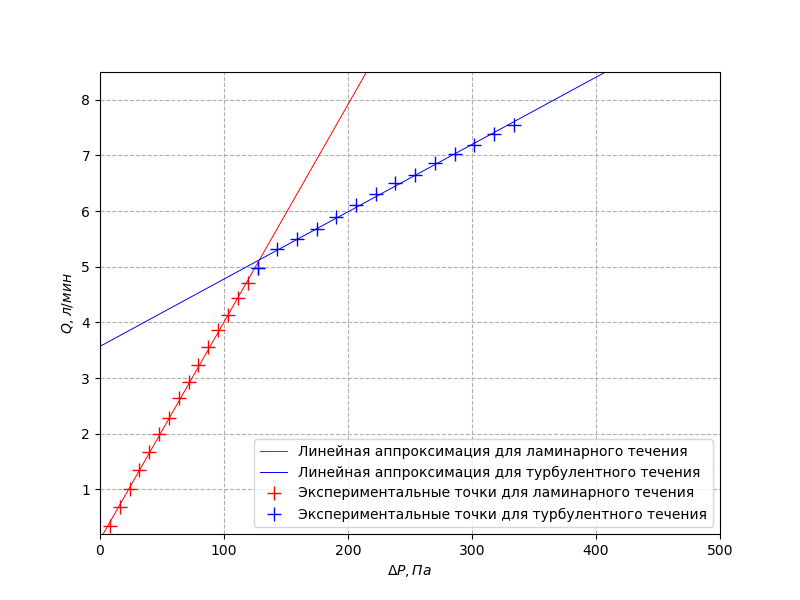
\includegraphics[width=1\textwidth]{graph_p-q_1.png}
	\caption{\textit{График зависимости $Q$ от $\Delta P$ для первой трубы}}
	\label{graph:p-q-1}
\end{figure}

\begin{figure}[h!]
        \centering
	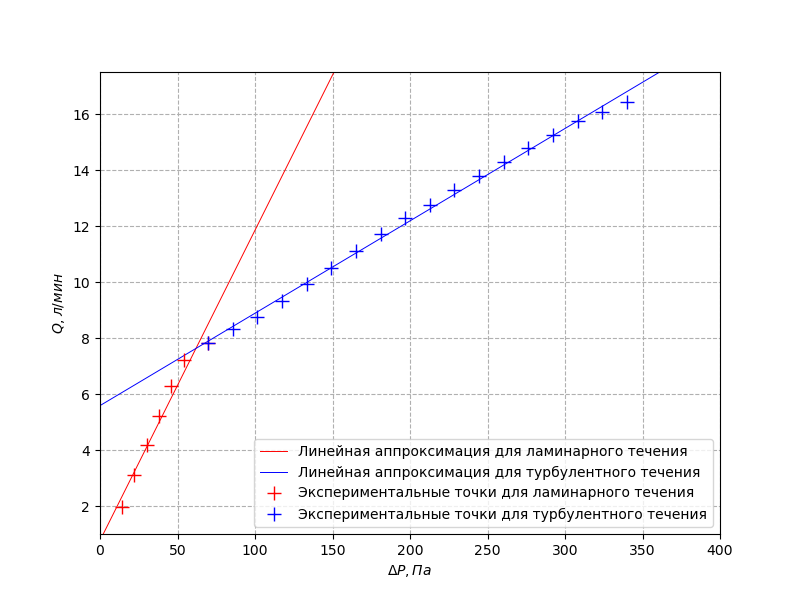
\includegraphics[width=1\textwidth]{graph_p-q_2.png}
	\caption{\textit{График зависимости $Q$ от $\Delta P$ для второй трубы}}
	\label{graph:p-q-2}
\end{figure}

\clearpage

Из формулы \eqref{2}, получаем

\begin{equation}
    Q = \frac{\pi r^4 \Delta P}{8 l \eta} \ \text{и} \ Q = k \Delta P \implies \eta = \frac{\pi r^4}{8 l k} = \frac{\pi d^4}{128 l k}
\end{equation}

Погрешность вычисления коэффициента вязкости можно вычислить по формуле:

\begin{equation*}
    \sigma_\eta = \sqrt{
    \left( \frac{\partial \eta}{\partial d} \right)^2 (\sigma_{d})^2 + 
    \left( \frac{\partial \eta}{\partial l} \right)^2 (\sigma_{l})^2 + 
    \left( \frac{\partial \eta}{\partial k} \right)^2 (\sigma_{k})^2
    } = 
\end{equation*}
\begin{equation}
    = \sqrt{
    \left(\frac{4 \eta}{d} \right)^2 \sigma_{d}^2 + 
    \left( \frac{\eta}{l} \right)^2 \sigma_{l}^2 + \left( \frac{\eta}{k} \right)^2 \sigma_{k}^2
    } = \eta \sqrt{
    16 \frac{\sigma_{d}^2}{d^2} + \frac{\sigma_{l}^2}{l^2} + \frac{\sigma_{k}^2}{k^2}
    }
\end{equation}

По этой формуле вычислим значение вязкости для обоих трубок:

\begin{equation*}
    \eta_1 = \frac{\pi r^4}{8 l k_1^\text{лам}} = \frac{3,14 \cdot ({3,90 \cdot 10^{-3} / 2})^4}{8 \cdot 0,5 \cdot 0,0391 / 60000} \approx 1,74 \cdot 10^{-5} \ \text{Па} \cdot \text{с}
\end{equation*}
\begin{equation*}
    \sigma_{\eta 1} = 1,7 \cdot 10^{-5} \sqrt{16 \frac{{0,05}^2}{{3,90}^2} + \frac{{0,5}^2}{{50,0}^2} + \frac{{0,003}^2}{{0,039}^2}} \approx 0,2 \cdot 10^{-5} \ \text{Па} \cdot \text{с}
\end{equation*}



\begin{equation*}
    \eta_2 = \frac{\pi r^4}{8 l k_2^\text{лам}} = \frac{3,14 \cdot ({5,25 \cdot 10^{-3} / 2})^4}{8 \cdot 0,5 \cdot 0,111 / 60000} \approx 2,0 \cdot 10^{-5} \ \text{Па} \cdot \text{с}
\end{equation*}
\begin{equation*}
    \sigma_{\eta 1} = 2,0 \cdot 10^{-5} \sqrt{16 \frac{{0,05}^2}{{3,90}^2} + \frac{{0,5}^2}{{50,0}^2} + \frac{{0,003}^2}{{0,039}^2}} \approx 0,2 \cdot 10^{-5} \ \text{Па} \cdot \text{с}
\end{equation*}

Видно, что полученные значения в пределах погрешности совпадают. Тогда вязкость равна:

\begin{equation}
    \eta = (1,85 \pm 0,2) \ \text{Па} \cdot \text{с}
\end{equation}

Теперь можем рассчитать критическое число Рейнольдса $Re_\text{кр}$:

\begin{equation*}
    Re_\text{кр} = \frac{Q_\text{кр} \rho}{\pi r \eta} = \frac{5 / 60000 \cdot 1,18}{3,14 \cdot (3,90 \cdot 10^{-3} / 2) \cdot 1,85 \cdot 10^{-5}} \approx 900
\end{equation*}

\subsection{Зависимость давления от координаты}

Построим график зависимости давления от координаты подключения микроманометра. При ламинарном тесении эта зависимость должна быть прямой, поэтому можем воспользовать МНК. В данном случае $x = \Delta P$, а $y = Q$. Для аппроксимации наилучшей прямой воспользуемся формулой:

\begin{equation}\label{eq:mnk}
    k = \frac{\langle xy\rangle - \langle x \rangle \langle y \rangle}{\langle x^2 \rangle - \langle x \rangle^2},
    \ \text{а} \ \  b = \langle y \rangle - k\langle x \rangle
\end{equation}

Погрешности для $k$ и $b$ рассчитываются по формулам:

\begin{equation}
    \sigma_k = \frac{1}{\sqrt{n}} \sqrt{\frac{\langle y^2 \rangle - \langle y \rangle^2}{\langle x^2 \rangle - \langle x \rangle^2} - k^2}
\end{equation}

\begin{equation}
    \sigma_b = \sigma_k\sqrt{\langle x^2 \rangle - \langle x \rangle^2}
\end{equation}
5
Посчитаем значение для точек ламинарного течения для обоих труб:

\begin{equation*}
    k_1 = \frac{3187,066 - 44,3 \cdot 63,5}{2787,67 - {44,3}^2} \approx 0,45 \ \text{Па}/\text{см}
\end{equation*}
\begin{equation*}
    b_1 = 63,5 - 0,45 \cdot 44,3 \approx 43,5 \ \text{па}
\end{equation*}
\begin{equation*}
    \sigma_{k1} = \frac{1}{\sqrt{3}} \sqrt{\frac{4204,172 - {63,5}^2}{2787,67 - {44,3}^2} - {0,45}^2} \approx 0,02 \ \text{Па}/\text{см}
\end{equation*}
\begin{equation*}
    \sigma_{b1} = 0,02 \sqrt{2787,67 - {44,3}^2} \approx 0,6 \ \text{Па}
\end{equation*}

\begin{equation*}
    k_2 = \frac{1289,121 - 43,8 \cdot 26,5}{2743,58 - {43,8}^2} \approx 0,16 \ \text{Па}/\text{см}
\end{equation*}
\begin{equation*}
    b_2 = 26,5 - 0,16 \cdot 43,8 \approx 19,6 \ \text{па}
\end{equation*}
\begin{equation*}
    \sigma_{k2} = \frac{1}{\sqrt{3}} \sqrt{\frac{721,436 - {26,5}^2}{2743,58 - {43,8}^2} - {0,16}^2} \approx 0,02 \ \text{Па}/\text{см}
\end{equation*}
\begin{equation*}
    \sigma_{b2} = 0,02 \sqrt{2743,58 - {43,8}^2} \approx 0,4 \ \text{Па}
\end{equation*}

Нанесём график для трубы 1 и для трубы 2 на рис. \ref{graph:p-x-1} и на рис. \ref{graph:p-x-2} соответственно.

\begin{figure}[h!]
        \centering
	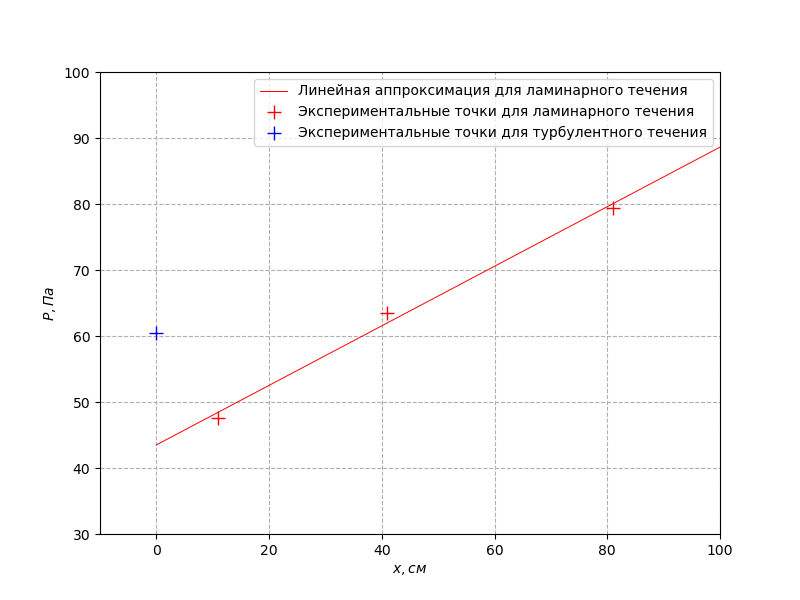
\includegraphics[width=1\textwidth]{graph_p-x_1.png}
	\caption{\textit{График зависимости $P$ от $x$ для первой трубы}}
	\label{graph:p-x-1}
\end{figure}

\begin{figure}[h!]
        \centering
	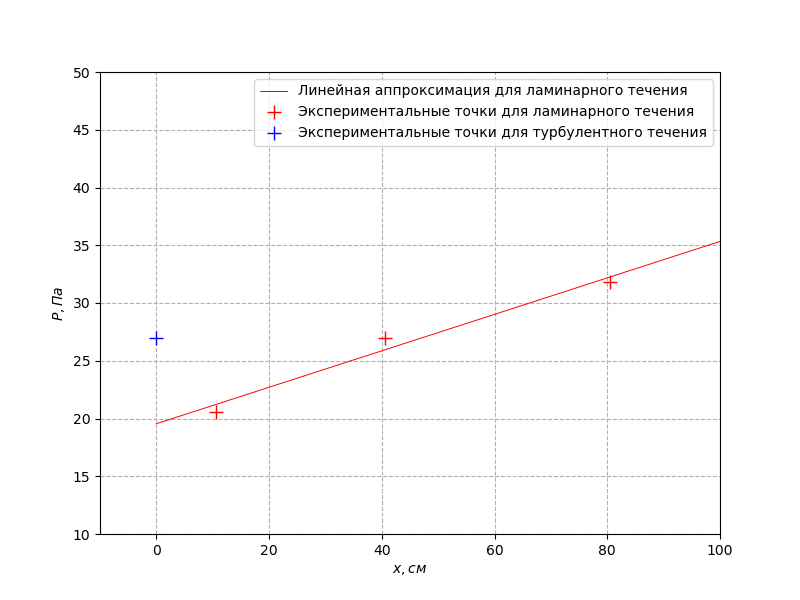
\includegraphics[width=1\textwidth]{graph_p-x_2.png}
	\caption{\textit{График зависимости $P$ от $x$ для второй трубы}}
	\label{graph:p-x-2}
\end{figure}

Из графиков видно, что значение $l_\text{уст}$ значительно меньше, чем теоретическое значение.

\clearpage

\subsection{Проверка зависимости расхода от радиуса}

Данный пункт работы не выполнялся, так как не выполнялся пункт \ref{p:10}.

\subsection{Зависимость $Q(\Delta P) на турбулентном участке$}

На турбулентном участке расход $Q$ должен линейно зависеть от $\sqrt{\Delta P r^5}$, для проверки этой зависимости воспользуемся МНК. В данном случае $x = \sqrt{\Delta P r^5}$, а $y = Q$. Параметры наилучшей прямой можно найти как:

\begin{equation}\label{eq:mnk-linear}
    k = \frac{\langle x y \rangle}{\langle x^2 \rangle}, \ \ \ \sigma_k = \frac{1}{\sqrt{n}} \sqrt{\frac{\langle y^2 \rangle}{\langle x^2 \rangle} - k^2}
\end{equation}

Посчитаем коэффициенты наилучшей прямой:

\begin{equation*}
    k = \frac{1361,819}{17204,738} \approx 0,0792 \ \frac{\text{л}}{\text{мин}} \cdot \frac{1}{\sqrt{\text{Па} \cdot \text{мм}^5}}
\end{equation*}
\begin{equation*}
    \sigma_k = \sigma_k = \frac{1}{\sqrt{32}} \sqrt{\frac{{107,825}^2}{{17204,738}^2} - {0,0792}^2} \approx 0,0002 \ \frac{\text{л}}{\text{мин}} \cdot \frac{1}{\sqrt{\text{Па} \cdot \text{мм}^5}}
\end{equation*}

Нанесём прямую и точки на рис. \ref{graph:q-pr}.

\begin{figure}[h!]
        \centering
	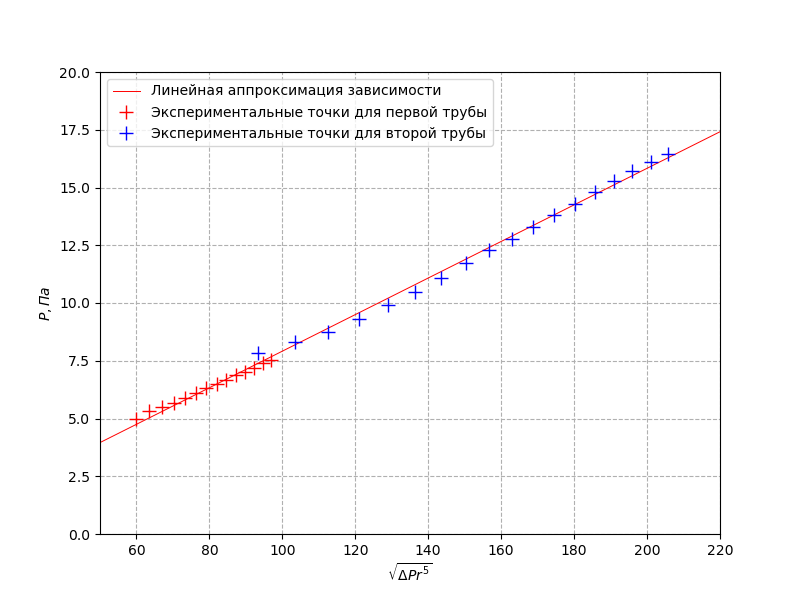
\includegraphics[width=1\textwidth]{graph_q-pr.png}
	\caption{\textit{График зависимости $Q$ от $\sqrt{\Delta P r^5}$}}
	\label{graph:q-pr}
\end{figure}

Из графика видно, что зависимость выполняется.


\section{Обсуждение результатов и выводы}

В ходе работы было эксперментально исследованы свойства течения газов по тонким трубкам при различных числах Рейнольдса. Было экспериментально получено значение вязкости газа в трубке.

Было исследованы зависимости для ламинарного и турбулентного течения.


\end{document}
